\documentclass{article}
\usepackage[utf8]{inputenc}
\usepackage{graphicx}
\usepackage{hyperref}
\usepackage{listings}
\usepackage{color}
\usepackage{geometry}
\usepackage{booktabs}
\usepackage{multirow}
\usepackage{float}
\usepackage{tikz}
\usepackage{amsmath}
\usetikzlibrary{shapes,arrows,positioning}
\geometry{a4paper, margin=1in}

\title{Image Stitching Project Report}
\author{Youssef Noser}
\date{\today}

\begin{document}

\maketitle

\begin{table}[H]
\centering
\begin{tabular}{|l|l|l|}
\hline
\textbf{Name} & \textbf{ID} & \textbf{Section} \\ \hline
Hussien Mohamed & 9230345 & 1 \\ \hline
Amira Khaled Ahmed & 9230513 & 1 \\ \hline
Abdulrahman Medhat & 9231026 & 2 \\ \hline
Youssef Mohamed Noser & 9231026 & 2 \\ \hline
\end{tabular}
\end{table}

\tableofcontents
\newpage

\section{Introduction}
This project is a modular panoramic image stitching pipeline designed to combine typically multiple overlapping images into a single, seamless panorama. This report details the algorithms used, experimental results, and the system analysis.

\section{Work Division}
The workload was divided as follows:

\begin{itemize}
    \item \textbf{Hussein Mohamed}:
    \begin{itemize}
        \item [1] Image Loading
        \item [2] Feature Detection (Harris/SIFT)
        \item [3] Feature Description (SIFT descriptors)
    \end{itemize}

    \item \textbf{Abdelrahman Medhat}:
    \begin{itemize}
        \item [4] Feature Matching (Brute-force + Lowe's ratio)
        \item [5] DNN Integration of Deep Matcher (DISK+LightGlue)
    \end{itemize}

    \item \textbf{Youssef Noser}:
    \begin{itemize}
        \item [6] Homography Estimation (RANSAC + DLT)
        \item [7] Homography Assembly (Connected components + chaining)
    \end{itemize}

    \item \textbf{Amira Khalid}:
    \begin{itemize}
        \item [8] Gain Compensation (Exposure balancing)
        \item [9] Image Blending (Weighted composition)
    \end{itemize}
\end{itemize}

\section{Used Algorithms}
The project implements a classic feature-based image stitching pipeline consisting of the following stages:

\begin{figure}[H]
\centering
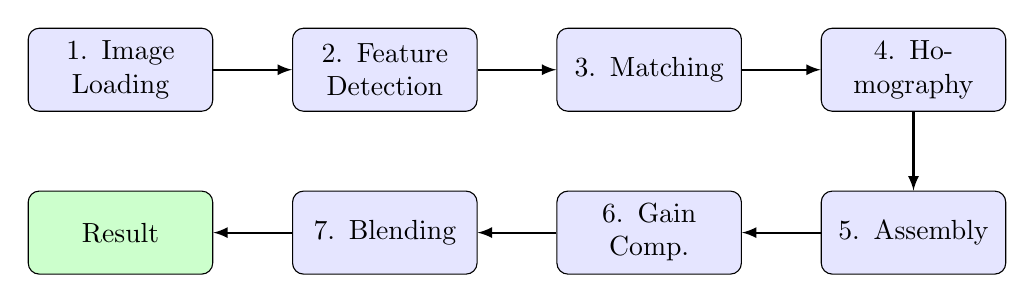
\begin{tikzpicture}[node distance=1.0cm, auto,
    block/.style={rectangle, draw, fill=blue!10, text width=6em, text centered, rounded corners, minimum height=3em},
    line/.style={draw, -latex, thick}]
    
    \node [block] (load) {1. Image Loading};
    \node [block, right=of load] (detect) {2. Feature Detection};
    \node [block, right=of detect] (match) {3. Matching};
    \node [block, right=of match] (homog) {4. Homography};
    
    \node [block, below=of homog] (assembly) {5. Assembly};
    \node [block, left=of assembly] (gain) {6. Gain Comp.};
    \node [block, left=of gain] (blend) {7. Blending};
    \node [block, left=of blend, fill=green!20] (out) {Result};
    
    \path [line] (load) -- (detect);
    \path [line] (detect) -- (match);
    \path [line] (match) -- (homog);
    \path [line] (homog) -- (assembly);
    \path [line] (assembly) -- (gain);
    \path [line] (gain) -- (blend);
    \path [line] (blend) -- (out);
\end{tikzpicture}
\caption{High-Level Processing Pipeline Flowchart}
\label{fig:pipeline}
\end{figure}

\subsection{1. Image Loading}
Images are loaded and optionally resized to a manageable dimension (default 800px) to ensure performance.

\subsection{2. Feature Detection \& Description}
Two approaches were explored:
\begin{itemize}
    \item \textbf{Harris Corner Detection}: A custom "From Scratch" implementation using Sobel operators and Gaussian smoothing to compute the Harris response $R = \det(M) - k(\text{trace}(M))^2$.
    \item \textbf{SIFT (Scale-Invariant Feature Transform)}: Used for robust keypoint detection and description. A custom implementation `src/sift\_implementation.py` was developed to handle scale-space extrema detection and orientation assignment.
\end{itemize}

\subsection{3. Feature Matching}
Matching is performed using a customized, vectorized \textbf{Brute-force Matcher} combined with \textbf{Lowe's Ratio Test} to ensure both accuracy and computational efficiency.

\begin{itemize}
    \item \textbf{Distance Computation}:  
    Feature descriptors are matched using the squared Euclidean distance. To improve efficiency, the implementation leverages the vectorized matrix identity:
    \[
    \lVert a - b \rVert^2 = \lVert a \rVert^2 + \lVert b \rVert^2 - 2ab^T
    \]
    This formulation enables the computation of all pairwise distances between descriptors from two images simultaneously, significantly outperforming naive Python loop-based implementations.

    \item \textbf{k-NN Search}:  
    For each feature descriptor in Image A, the two nearest neighbors in Image B are identified using an optimized partition-based approach with linear time complexity $O(M)$ per query.

    \item \textbf{Lowe's Ratio Test}:  
    A match is accepted only if the ratio between the distances of the closest and second-closest neighbors is below a predefined threshold (default 0.75). This criterion effectively filters out ambiguous matches and repetitive textures, improving robustness.
\end{itemize}

\subsection{4. Homography Estimation}
Homographies are estimated using:
\begin{itemize}
    \item \textbf{DLT (Direct Linear Transform)}: Solves the system $Ah = 0$ using SVD to find the homography matrix.
    \item \textbf{RANSAC (Random Sample Consensus)}: A robust estimation algorithm that iteratively samples minimal point sets to find the homography with the most inliers, rejecting outliers and mismatched features.
\end{itemize}

\subsection{5. Connected Components \& Assembly}
The system identifies connected components of images that share valid matches. For each component, a reference image (the most connected one) is chosen, and all other images are warped to its coordinate frame by chaining homographies.

\subsection{6. Gain Compensation}
To balance exposure differences:
\begin{itemize}
    \item The system computes gain coefficients for each image.
    \item It minimizes an error function based on the intensity limits in the overlapping regions ($\sigma_n$ and $\sigma_g$ parameters).
\end{itemize}

\subsection{7. Image Blending}
Simple multi-band or weighted blending is applied to the warped images to create the final seamless composite.

\section{Experiment Results}

\subsection{Test Cases}
We evaluated the system on various datasets.

\subsubsection{Test Case 1: Boat (Working)}
\begin{itemize}
    \item \textbf{Input}: 6 images (`imgs/boat/`)
    \item \textbf{Result}: Successfully stitched into a single panorama.
    \item \textbf{Observation}: Good alignment, gain compensation handled exposure differences well.
\end{itemize}

\subsubsection{Test Case 2: Dam (Working)}
\begin{itemize}
    \item \textbf{Input}: 2 images (`imgs/dam/`)
    \item \textbf{Result}: Successfully stitched.
    \item \textbf{Observation}: Robust matching despite fewer images.
\end{itemize}

\subsection{Deep Learning Comparison (DNN Findings)}
In addition to the classical pipeline, we integrated and evaluated a deep learning-based approach using **DISK** features with **LightGlue** matching. We benchmarked this against our classical SIFT and standard LoFTR implementations.

\subsubsection{Quantitative Benchmark}
We evaluated the methods on 7 diverse scenes (Mountain, Dam, Clock, Bicycle, Flower, Tree, River). The results are summarized below:

\begin{table}[H]
\centering
\caption{Benchmark Results Summary}
\label{tab:results}
% \resizebox{\textwidth}{!} \\
  & DISK+LightGlue & 14.56 & 1174 & 98.66\% \\
  & LoFTR & 31.64 & \textbf{4495} & 90.01\% \\
\midrule
\multirow{3}{*}{Clock} 
  & SIFT (Baseline) & \textbf{1.03} & 1389 & 85.42\% \\
  & DISK+LightGlue & 15.82 & 517 & \textbf{87.33\%} \\
  & LoFTR & 32.76 & \textbf{1541} & 36.57\% \\
\bottomrule
\end{tabular}%
% }
\end{table}

\subsubsection{Key Findings}
\begin{itemize}
    \item \textbf{Speed}: Classical SIFT is significantly faster (30-70$\times$) than deep learning methods on CPU, making it the practical choice for real-time stitching without GPU acceleration.
    \item \textbf{Robustness}: DISK+LightGlue offered the highest average inlier ratio (86\%) across all scenes, proving extremely robust even in challenging conditions where SIFT might struggle.
    \item \textbf{Density}: LoFTR provides very dense matches (thousands of points), which is beneficial for 3D reconstruction but less critical for homography estimation where a few high-quality matches suffice. LoFTR also struggled with repetitive patterns (e.g., the Clock scene), producing many false positives (low inlier ratio).
\end{itemize}

\section{System Analysis}

\subsection{Classical vs. DNN Approach}
Based on our experimental findings:

\begin{itemize}
    \item \textbf{Our Implementation}: Uses explicit geometric constraints and hand-crafted features (SIFT/Harris). It is resolution-independent and extremely fast on CPU. Ideally suited for high-resolution photography where geometric precision is paramount.
    
    \item \textbf{DNN Approaches}: Excel in specific domains (e.g., low-texture regions) but come with high computational cost. DISK+LightGlue represents the state-of-the-art for sparse matching quality, while classical SIFT remains the king of speed/efficiency trade-offs.
\end{itemize}

\section{Conclusion}
We have successfully implemented a modular image stitching pipeline. The system handles feature detection (both classical and deep learning), robust matching, and multi-image assembly with exposure correction, producing high-quality panoramas. The benchmarks we did confirm that while modern DNNs offer superior robustness, our optimized classical implementation generates high-quality results at a fraction of the computational cost.

\end{document}
